\cleardoublepage
% Kapitel Fallbeispiel Zoo: über das Marko werden Kapitel, Eintrag Inhaltsverzeichnis und die Kopfzeilen konfiguriert.
\FallBeispielZoo
\label{sec:Lektion-2-Zoo}

\marginline{~\\Lektion~1, Seite~\pageref*{sec:Lektion-1-Zoo}}
\sttpUniversalkasten{Was bisher geschah}{Der städtische Zoo ist an das Softwareunternehmen herangetreten, in dem Sie arbeiten, um zu eruieren, an welchen Stellen Zooabläufe mit Software unterstützt werden könnten und wie der öffentliche Zooauftritt insgesamt digitaler werden kann. Welche Dienstleistungen der Zoo von Ihrem Unternehmen erwartet, ist aktuell noch recht vage. \newline \newline	
Wir befinden uns in einer ersten Brainstorming-Besprechung zwischen dem Softwareentwicklungsteam und einer Abordnung des Zoos. Frau Dr. Walther, die Zoodirektorin, hat soeben in einem sehr informationsdichten Rundumschlag zur Domäne Zoo erzählt und dabei auch erste Andeutungen gemacht, für welche Aspekte sie sich Softwareunterstützung vorstellen könnte.}

\minisec{Die Besprechung wird fortgesetzt}

Ihr Chef, Herr Steiber, bedankt sich bei der Zoodirektorin für ihre Ausführungen. Im Anschluss wird frei diskutiert, es wird nachgefragt, zusätzliche Informationen werden erteilt, Unklarheiten angesprochen, manches konkretisiert, anderes im Vagen gelassen, weitere Wünsche geäußert, jede und jeder macht sich ein paar Notizen,~\ldots 
\linebreak
Auf diese Weise sind schnell zwei Stunden vergangen. Die Chemie scheint zu stimmen zwischen dem Zoo- und dem Softwareentwicklungsteam.

Herr Steiber und die Zoodirektorin haben dann auch zwischenzeitlich eine Kaffeepause genutzt, um sich grundsätzlich auf die Zusammenarbeit zu verständigen. Man definiert die heutige Besprechung als Beginn eines kleineren Vorprojekts, in dem der inhaltliche und zeitliche Rahmen für das hoffentlich anschließende eigentliche Softwareentwicklungsprojekt verhandelt wird. Herr Steiber konnte der Zoo\-direk\-torin auch schon mal vorsichtig nahebringen, dass es sicher nicht auf eine allumfassende vollintegrierte und automatisierte Zooverwaltungs- und Zoodigitalisierungssoftware hinauslaufen wird.

\textbf{Hr. Steiber:} „Ich darf um Ihre Aufmerksamkeit bitten! Schön, dass wir schon so intensiv ins Diskutieren gekommen sind. Wir sollten unseren Austausch jetzt aber etwas systematisieren und vor allem unsere Gedanken festhalten. Daher bitte ich Sie, auf den Karteikarten die noch offenen Fragen zur Domäne zu notieren. Erstellen Sie dort bitte auch kurze Beschreibungen der Zoo-Abläufe und -Aufgaben, über die wir hier gerade diskutiert hatten. Einige von Ihnen hatten sich vorhin zudem schon erste Gedanken über das zukünftige Softwareprodukt gemacht, halten Sie das bitte auch alles auf den Karteikarten fest. Und Kollege Fryt, beginnen Sie doch bitte parallel schon mal mit einem ersten groben Domänenklassendiagramm, Sie sehen ja, welche Informationen zur Domäne die anderen ans Whiteboard heften. Aber verlieren Sie sich bloß noch nicht im Detail, da wird es sicher noch viele Änderungen geben, wenn wir uns weiter über die Domäne austauschen.“

\minisec{Einige Zeit später}

% Anmerkung: man kann die Verweise noch wie gewünscht anpassen. Wenn der Verweis hinter den Grafiken stört (roter Rahmen), dann nimmt man "\hyperref[...]{}" weg und lässt nur den 2. Parameter in der geschweiften Klammer stehen. Bei den Bildunterschriften kann man ebenfalls frei entscheiden, wie es aussehen soll.

\begin{center}
	\begin{minipage}[c]{.65\linewidth}
		\centering
		\hyperref[text:lektion2_whiteboard_s1]{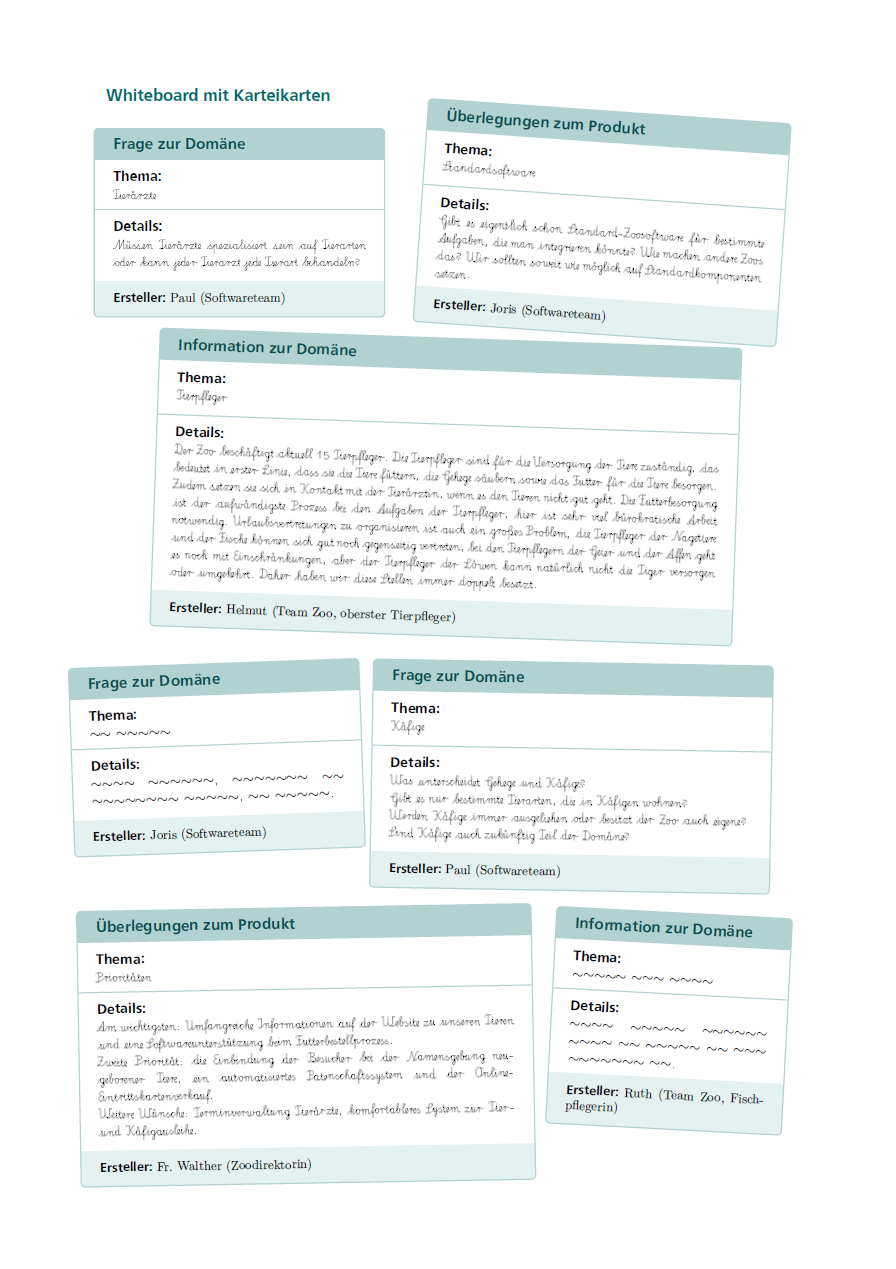
\includegraphics[width=0.45\linewidth]{Bilder/Zoo/whiteboard_s1.png} 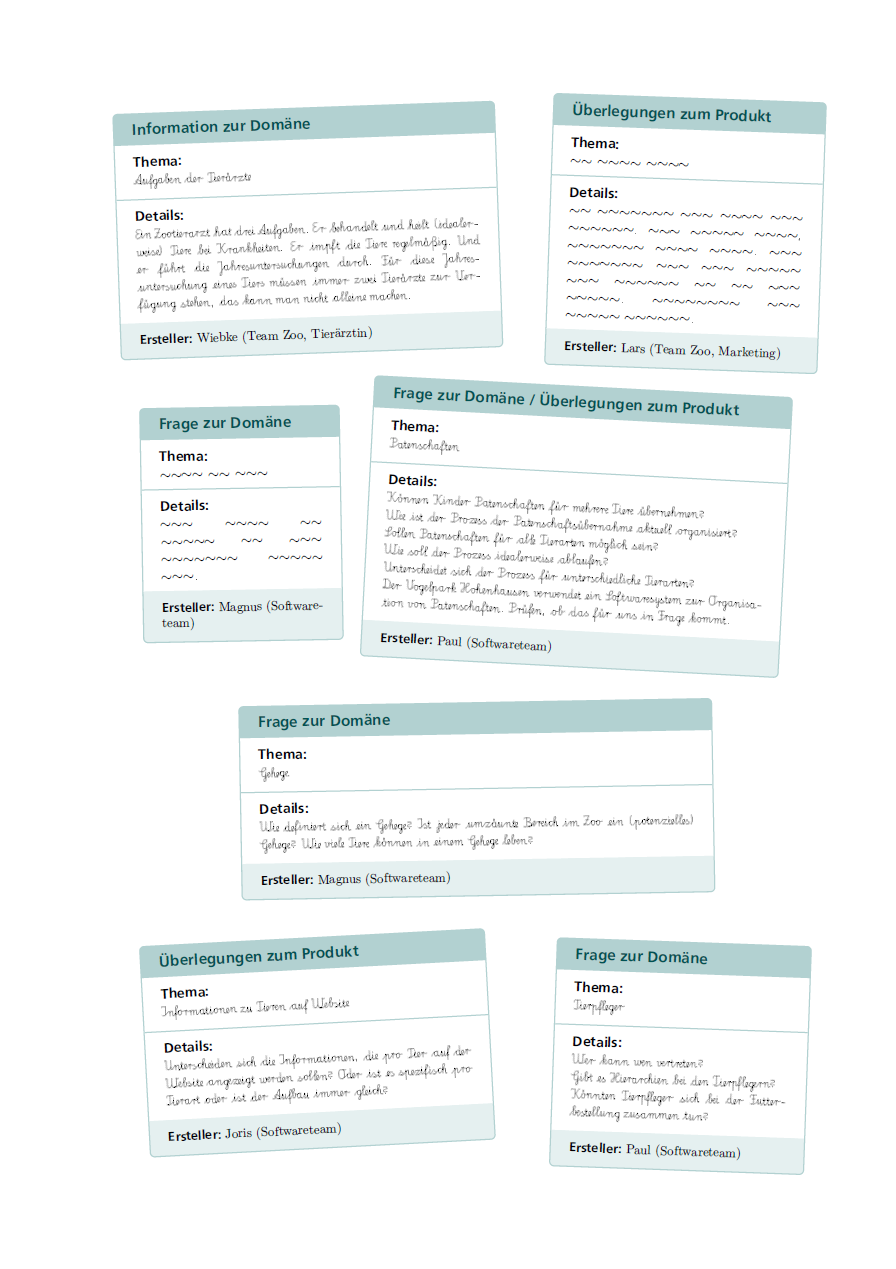
\includegraphics[width=0.45\linewidth]{Bilder/Zoo/whiteboard_s2.png}}
		Whiteboard mit Karteikarten (vergrößerte Darstellung auf Seite~\pageref{text:lektion2_whiteboard_s1}f.)
	\end{minipage}
	\hspace{0.1cm}% Abstand zwischen den beiden Bildern
	\begin{minipage}[c]{.33\linewidth}
		\centering
		\hyperref[fig:lektion2_fallbeispiel_zoo]{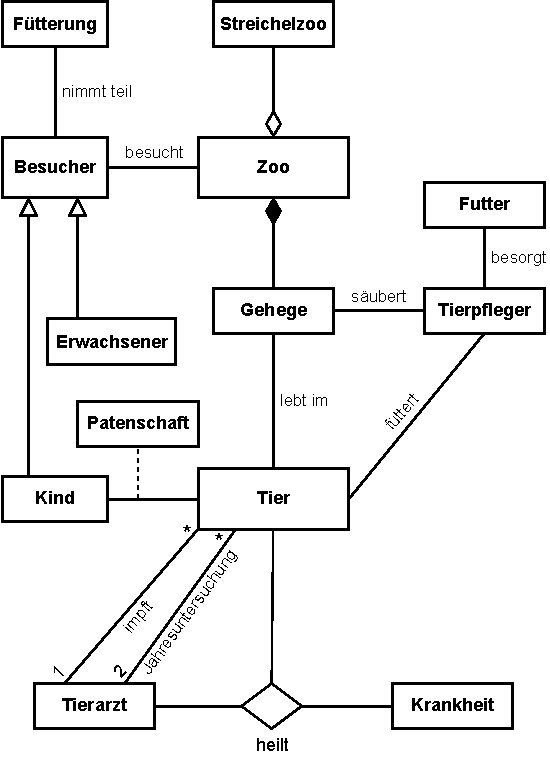
\includegraphics[width=\linewidth]{Bilder/Zoo/fallbeispiel_zoo.pdf}}
		Domänenklassendiagramm Zoo (vergrößert in Abbildung~\ref{fig:lektion2_fallbeispiel_zoo})
	\end{minipage}
\end{center}

\textbf{Hr. Steiber:} „Ich danke Ihnen allen! Für das erste Treffen waren wir doch schon sehr produktiv. Sie haben ja schon mitbekommen, dass mit diesem Treffen unser Vorprojekt nun offiziell gestartet ist. Wir werden uns in den nächsten Tagen und Wochen in kleineren Runden wieder treffen und zum einen an der Modellierung der Domäne weiterarbeiten und zum anderen uns natürlich über den Inhalt des zu entwickelnden Softwareprodukts Gedanken machen. Die Kollegin Schwab wird als sehr erfahrene Projektleiterin die Leitung des Vorprojekts übernehmen und zeitnah die verschiedenen Arbeitsgruppen einteilen. Für heute beende ich die Besprechung und wünsche uns allen einen schönen Feierabend.“

\minisec{Am nächsten Tag im Softwareunternehmen}
Die drei Kolleg:innen Inga Schwab (Projektleiterin Vorprojekt), Magnus Fryt (Requirement Engineer) und Joris Jonson (Softwarearchitekt) sitzen zusammen und planen die nächsten Schritte.

\textbf{Inga Schwab:} „Die Domäne Zoo ist komplexer, als ich das gedacht hatte. Unser aktuelles Domänenmodell ist noch viel zu grob. Lasst uns zunächst mal bei der Klasse Tier und der Klasse Tierpfleger ansetzen. Diese Informationen werden wir in jedem Fall brauchen, unabhängig davon, auf welche Aufgabenbereiche für das Softwareprodukt wir uns einigen. Tier scheint nicht gleich Tier zu sein. Ich habe den Eindruck, dass Strukturen und Abläufe der Domäne durchaus unterschiedlich aussehen, je nachdem über welche Tierart wir sprechen. Und auch bei den Tier\-pflegern scheinen Arbeitsabläufe davon abhängig zu sein, welche Tierarten sie betreuen. Was mir gestern, trotz der umfangreichen Erklärungsversuche des Zoo-Teams, bis zum Schluss nicht klar geworden ist, warum es einen auf Löwen spezialisierten Tier\-pfleger geben muss und einen anderen Tierpfleger für die Tiger, die Nagetiere und die Fische aber vom selben Tierpfleger versorgt werden können. Möglicherweise ist das nur historisch so gewachsen im Zoo, aber wir müssen sicher sein, dass uns hier nicht grundlegende Restriktionen der Domäne entgehen. Magnus, übernimm du bitte die Leitung der Arbeitsgruppe Domänenmodellierung. Hol dir Paul dazu, er hat sich in der Besprechung gestern schon gut in die Domäne herein gedacht. Von der Zooseite aus versuche ich dir zwei bis drei der Tierpfleger für die Arbeitsgruppe zu organisieren. Joris, du und ich werden uns mit der Zoo-Führung zusammensetzen und in die Entwicklungsplanung einsteigen, erste Prioritäten hat Frau Dr. Walther ja gestern immerhin schon gesetzt.“

% Das Whiteboard wird auf 2 Seiten dargestellt und soll somit auf einer linken Seite beginnen.
\cleardoubleevenemptypage 

\newgeometry{left=25mm, right=15mm, top=20mm, bottom=20mm,
	marginparwidth=5mm, marginparsep=1mm}
%TODO @Maren: Falls diese Seite wieder eine Kopfzeile haben soll, muss die folgende Zeile - \thispagestyle{empty} - auskommenitert werden.
\thispagestyle{empty}

\phantomsection
\label{text:lektion2_whiteboard_s1}
\minisec{\hspace{1cm}Whiteboard mit Karteikarten}

%\begin{figure}[h!]

{ %% Scope beginnen (damit \renewcommand keine Auswirkung auf andere Karteikarten hat)
	\setlength{\unitlength}{1mm}
	\renewcommand{\sttpKarteikarteSkalierungsfaktor}{0.85}
	
	\begin{picture}(0,0)
		\put(-35,-44){
			\renewcommand{\sttpKarteikarteRotierungswinkel}{0}
			% Karteikarte Fallbeispiel Zoo

\sttpKarteikarte{8cm}{\sttpKarteikarteSkalierungsfaktor}{\sttpKarteikarteRotierungswinkel}{Frage zur Domäne}%
	{Thema:}{Tierärzte}%
	{Details:}{Müssen Tierärzte spezialisiert sein auf Tierarten oder kann jeder Tierarzt jede Tierart behandeln?}%
	{Paul (Softwareteam)}

		}
		\put(48,-45){
			\renewcommand{\sttpKarteikarteRotierungswinkel}{-4}
			% Karteikarte Fallbeispiel Zoo

\sttpKarteikarte{10cm}{\sttpKarteikarteSkalierungsfaktor}{\sttpKarteikarteRotierungswinkel}{Überlegungen zum Produkt}%
	{Thema:}{Standardsoftware}%
	{Details:}{Gibt es eigentlich schon Standard-Zoosoftware für bestimmte Aufgaben, die man integrieren könnte? Wie machen andere Zoos das? Wir sollten soweit wie möglich auf Standardkomponenten setzen.}%
	{Joris (Softwareteam)}

		}
		\put(12,-116){
			\renewcommand{\sttpKarteikarteRotierungswinkel}{-2}
			% Karteikarte Fallbeispiel Zoo

\sttpKarteikarte{16cm}{\sttpKarteikarteSkalierungsfaktor}{\sttpKarteikarteRotierungswinkel}{Information zur Domäne}%
	{Thema:}{Tierpfleger}%
	{Details:}{Der Zoo beschäftigt aktuell 15 Tierpfleger. Die Tierpfleger sind für die Versorgung der Tiere zuständig, das bedeutet in erster Linie, dass sie die Tiere füttern, die Gehege säubern sowie das Futter für die Tiere besorgen. Zudem setzen sie sich in Kontakt mit der Tierärztin, wenn es den Tieren nicht gut geht. Die Futterbesorgung ist der aufwändigste Prozess bei den Aufgaben der Tierpfleger, hier ist sehr viel bürokratische Arbeit notwendig. Urlaubsvertretungen zu organisieren ist auch ein großes Problem, die Tierpfleger der Nagetiere und der Fische können sich gut noch gegenseitig vertreten, bei den Tierpflegern der Geier und der Affen geht es noch mit Einschränkungen, aber der Tierpfleger der Löwen kann natürlich nicht die Tiger versorgen oder umgekehrt. Daher haben wir diese Stellen immer doppelt besetzt.}%
	{Helmut (Team Zoo, oberster Tierpfleger)}

		}
		\put(-41,-170){
			\renewcommand{\sttpKarteikarteRotierungswinkel}{2}
			% Diese Karteikarte kann als Vorlage dienen

\sttpKarteikarte{8cm}{\sttpKarteikarteSkalierungsfaktor}{\sttpKarteikarteRotierungswinkel}{Frage zur Domäne}%
{Thema:}{$\sim$$\sim$ $\sim$$\sim$$\sim$$\sim$$\sim$}%
{Details:}{$\sim$$\sim$$\sim$$\sim$ $\sim$$\sim$$\sim$$\sim$$\sim$$\sim$, $\sim$$\sim$$\sim$$\sim$$\sim$$\sim$$\sim$ $\sim$$\sim$ $\sim$$\sim$$\sim$$\sim$$\sim$$\sim$$\sim$$\sim$ $\sim$$\sim$$\sim$$\sim$$\sim$, $\sim$$\sim$ $\sim$$\sim$$\sim$$\sim$$\sim$.}
{Joris (Softwareteam)}
		}
		\put(42,-177){
			\renewcommand{\sttpKarteikarteRotierungswinkel}{-1}
			% Karteikarte Fallbeispiel Zoo

\sttpKarteikarte{11cm}{\sttpKarteikarteSkalierungsfaktor}{\sttpKarteikarteRotierungswinkel}{Frage zur Domäne}%
	{Thema:}{Käfige}%
	{Details:}{Was unterscheidet Gehege und Käfige? \newline Gibt es nur bestimmte Tierarten, die in Käfigen wohnen? \newline Werden Käfige immer ausgeliehen oder besitzt der Zoo auch eigene? \newline Sind Käfige auch zukünftig Teil der Domäne?}%
	{Paul (Softwareteam)}
		}
		\put(64,-232){
			\renewcommand{\sttpKarteikarteRotierungswinkel}{-3}
			% Diese Karteikarte kann als Vorlage dienen

\sttpKarteikarte{6.5cm}{\sttpKarteikarteSkalierungsfaktor}{\sttpKarteikarteRotierungswinkel}{Information zur Domäne}%
	{Thema:}{$\sim$$\sim$$\sim$$\sim$$\sim$ $\sim$$\sim$$\sim$ $\sim$$\sim$$\sim$$\sim$}%
	{Details:}{$\sim$$\sim$$\sim$$\sim$ $\sim$$\sim$$\sim$$\sim$$\sim$ $\sim$$\sim$$\sim$$\sim\sim\sim$ $\sim\sim\sim\sim$ $\sim$$\sim$ $\sim$$\sim$$\sim$$\sim$$\sim$ $\sim$$\sim$ $\sim$$\sim$$\sim$ $\sim$$\sim$$\sim$$\sim$$\sim$$\sim$$\sim$ $\sim$$\sim$.}
	{Ruth (Team Zoo, Fischpflegerin)}
		}
		\put(-20,-247){
			\renewcommand{\sttpKarteikarteRotierungswinkel}{1}
			% Karteikarte Fallbeispiel Zoo

\sttpKarteikarte{12.5cm}{\sttpKarteikarteSkalierungsfaktor}{\sttpKarteikarteRotierungswinkel}{Überlegungen zum Produkt}%
	{Thema:}{Prioritäten}%
	{Details:}{Am wichtigsten: Umfangreiche Informationen auf der Website zu unseren Tieren und eine Softwareunterstützung beim Futterbestellprozess. \newline Zweite Priorität: die Einbindung der Besucher bei der Namensgebung neugeborener Tiere, ein automatisiertes Patenschaftssystem und der Online-Eintrittskartenverkauf. \newline Weitere Wünsche: Terminverwaltung Tierärzte, komfortableres System zur Tier- und Käfigausleihe.}%
	{Fr. Walther (Zoodirektorin)}
	
	
	

		}
	\end{picture}
} %% Scope beenden (um \renewcommand lokal zu halten)

%\caption{Whiteboard}
%\label{fig:lektion2_whiteboard_s1}
%\end{figure}

\restoregeometry

\clearpage

\newgeometry{left=25mm, right=15mm, top=20mm, bottom=20mm,
	marginparwidth=5mm, marginparsep=1mm}
%TODO @Maren: Falls diese Seite wieder eine Kopfzeile haben soll, muss die folgende Zeile - \thispagestyle{empty} - auskommenitert werden.
\thispagestyle{empty}

\phantomsection
\label{text:lektion2_whiteboard_s2}
% Keine Überschrift hier, aber selben Platz verbrauchen ;-)
\minisec{~~~}

%\begin{figure}[h!]

{ %% Scope beginnen (damit \renewcommand keine Auswirkung auf andere Karteikarten hat)
	\setlength{\unitlength}{1mm}
	\renewcommand{\sttpKarteikarteSkalierungsfaktor}{0.85}
	
	\begin{picture}(0,0)
		\put(-30,-54){
			\renewcommand{\sttpKarteikarteRotierungswinkel}{2}
			% Karteikarte Fallbeispiel Zoo

\sttpKarteikarte{10.5cm}{\sttpKarteikarteSkalierungsfaktor}{\sttpKarteikarteRotierungswinkel}{Information zur Domäne}%
	{Thema:}{Aufgaben der Tierärzte}%
	{Details:}{Ein Zootierarzt hat drei Aufgaben. Er behandelt und heilt (idealer\-weise) Tiere bei Krankheiten. Er impft die Tiere regelmäßig. Und er führt die Jahresuntersuchungen durch. Für diese Jahres\-untersuchung eines Tiers müssen immer zwei Tierärzte zur Verfügung stehen, das kann man nicht alleine machen.}%
	{Wiebke (Team Zoo, Tierärztin)}

		}
		\put(58,-55){
			\renewcommand{\sttpKarteikarteRotierungswinkel}{-2}
			% Diese Karteikarte kann als Vorlage dienen

\sttpKarteikarte{7.5cm}{\sttpKarteikarteSkalierungsfaktor}{\sttpKarteikarteRotierungswinkel}{Überlegungen zum Produkt}%
	{Thema:}{$\sim$$\sim$ $\sim$$\sim$$\sim$$\sim$ $\sim$$\sim$$\sim$$\sim$}%
	{Details:}{$\sim$$\sim$ $\sim$$\sim$$\sim$$\sim$$\sim$$\sim$$\sim$ $\sim$$\sim$$\sim$ $\sim$$\sim$$\sim$$\sim$ $\sim$$\sim$$\sim$ $\sim$$\sim$$\sim$$\sim$$\sim$$\sim$. $\sim$$\sim$$\sim$ $\sim$$\sim$$\sim$$\sim$$\sim$ $\sim$$\sim$$\sim$$\sim$, $\sim$$\sim$$\sim$$\sim$$\sim$$\sim$$\sim$ $\sim$$\sim$$\sim$$\sim$ $\sim$$\sim$$\sim$$\sim$. $\sim$$\sim$$\sim$ $\sim$$\sim$$\sim$$\sim$$\sim$$\sim$$\sim$ $\sim$$\sim$$\sim$ $\sim$$\sim$$\sim$ $\sim$$\sim$$\sim$$\sim$$\sim$ $\sim$$\sim$$\sim$ $\sim$$\sim$$\sim$$\sim$$\sim$$\sim$ $\sim$$\sim$ $\sim$$\sim$ $\sim$$\sim$$\sim$ $\sim$$\sim$$\sim$$\sim$$\sim$. $\sim$$\sim$$\sim$$\sim$$\sim$$\sim$$\sim$$\sim$ $\sim$$\sim$$\sim$ $\sim$$\sim$$\sim$$\sim$$\sim$ $\sim$$\sim$$\sim$$\sim\sim\sim$.}
	{Lars (Team Zoo, Marketing)}
		}
		\put(32,-123){
			\renewcommand{\sttpKarteikarteRotierungswinkel}{-3}
			% Karteikarte Fallbeispiel Zoo

\sttpKarteikarte{11.5cm}{\sttpKarteikarteSkalierungsfaktor}{\sttpKarteikarteRotierungswinkel}{Frage zur Domäne / Überlegungen zum Produkt}%
	{Thema:}{Patenschaften}%
	{Details:}{Können Kinder Patenschaften für mehrere Tiere übernehmen? \newline Wie ist der Prozess der Patenschaftsübernahme aktuell organisiert? \newline Sollen Patenschaften für alle Tierarten möglich sein? \newline Wie soll der Prozess idealerweise ablaufen? \newline Unterscheidet sich der Prozess für unterschiedliche Tierarten? \newline Der Vogelpark Hohenhausen verwendet ein Softwaresystem zur Organisation von Patenschaften. Prüfen, ob das für uns in Frage kommt.}%
	{Paul (Softwareteam)}

		}
		\put(10,-180){
			\renewcommand{\sttpKarteikarteRotierungswinkel}{1}
			% Karteikarte Fallbeispiel Zoo

\sttpKarteikarte{13cm}{\sttpKarteikarteSkalierungsfaktor}{\sttpKarteikarteRotierungswinkel}{Frage zur Domäne}%
	{Thema:}{Gehege}%
	{Details:}{Wie definiert sich ein Gehege? Ist jeder umzäunte Bereich im Zoo ein (potenzielles) Gehege? Wie viele Tiere können in einem Gehege leben?}%
	{Magnus (Softwareteam)}

		}
		\put(-28,-240){
			\renewcommand{\sttpKarteikarteRotierungswinkel}{3}
			% Karteikarte Fallbeispiel Zoo

\sttpKarteikarte{9.5cm}{\sttpKarteikarteSkalierungsfaktor}{\sttpKarteikarteRotierungswinkel}{Überlegungen zum Produkt}%
	{Thema:}{Informationen zu Tieren auf Website}%
	{Details:}{Unterscheiden sich die Informationen, die pro Tier auf der Website angezeigt werden sollen? Oder ist es spezifisch pro Tierart oder ist der Aufbau immer gleich?}%
	{Joris (Softwareteam)}

		}
		\put(-45,-120){
			\renewcommand{\sttpKarteikarteRotierungswinkel}{1}
			% Diese Karteikarte kann als Vorlage dienen

\sttpKarteikarte{5.5cm}{\sttpKarteikarteSkalierungsfaktor}{\sttpKarteikarteRotierungswinkel}{Frage zur Domäne}%
	{Thema:}{$\sim$$\sim$$\sim$$\sim$ $\sim$$\sim$ $\sim$$\sim$$\sim$}%
	{Details:}{$\sim\sim\sim$ $\sim\sim\sim\sim$ $\sim$$\sim$ $\sim$$\sim$$\sim$$\sim$$\sim$ $\sim$$\sim$ $\sim$$\sim$$\sim$ $\sim$$\sim$$\sim$$\sim$$\sim$$\sim$$\sim$ $\sim$$\sim$$\sim$$\sim$$\sim$ $\sim$$\sim$$\sim$.}
	{Magnus (Softwareteam)}
		}
		\put(57,-242){
			\renewcommand{\sttpKarteikarteRotierungswinkel}{-2}
			% Karteikarte Fallbeispiel Zoo

\sttpKarteikarte{7cm}{\sttpKarteikarteSkalierungsfaktor}{\sttpKarteikarteRotierungswinkel}{Frage zur Domäne}%
	{Thema:}{Tierpfleger}%
	{Details:}{Wer kann wen vertreten? \newline Gibt es Hierarchien bei den Tierpflegern? \newline Könnten Tierpfleger sich bei der Futter\-bestellung zusammen tun?}%
	{Paul (Softwareteam)}

		}
		%		\put(-20,-247){
			%			\renewcommand{\sttpKarteikarteRotierungswinkel}{1}
			%			\input{Karteikarten/xxx.tex}
			%		}
	\end{picture}
} %% Scope beenden (um \renewcommand lokal zu halten)

%\caption{Whiteboard}
%\label{fig:lektion2_whiteboard_s2}
%\end{figure}

\restoregeometry

\clearpage

\vspace*{4cm} %%% Abbildung auf Seite zentrieren

\begin{figure}[h!]
	\centering
	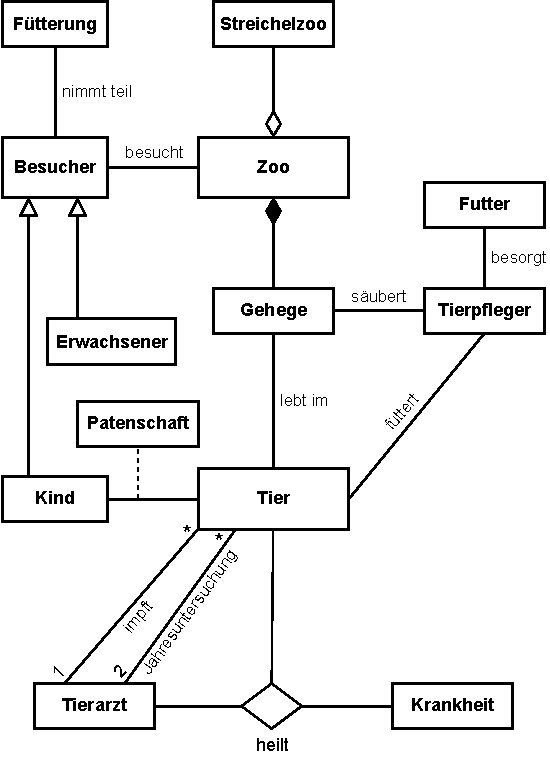
\includegraphics{Bilder/Zoo/fallbeispiel_zoo.pdf}
	\caption{Domänenklassendiagramm für den Zoo}
	\label{fig:lektion2_fallbeispiel_zoo}
\end{figure}